\section{Finite State Automata (FSA) Design} \label{section: fsa design}
The following describes the Secret Door Logic through an FSA illustration and a description: \\
{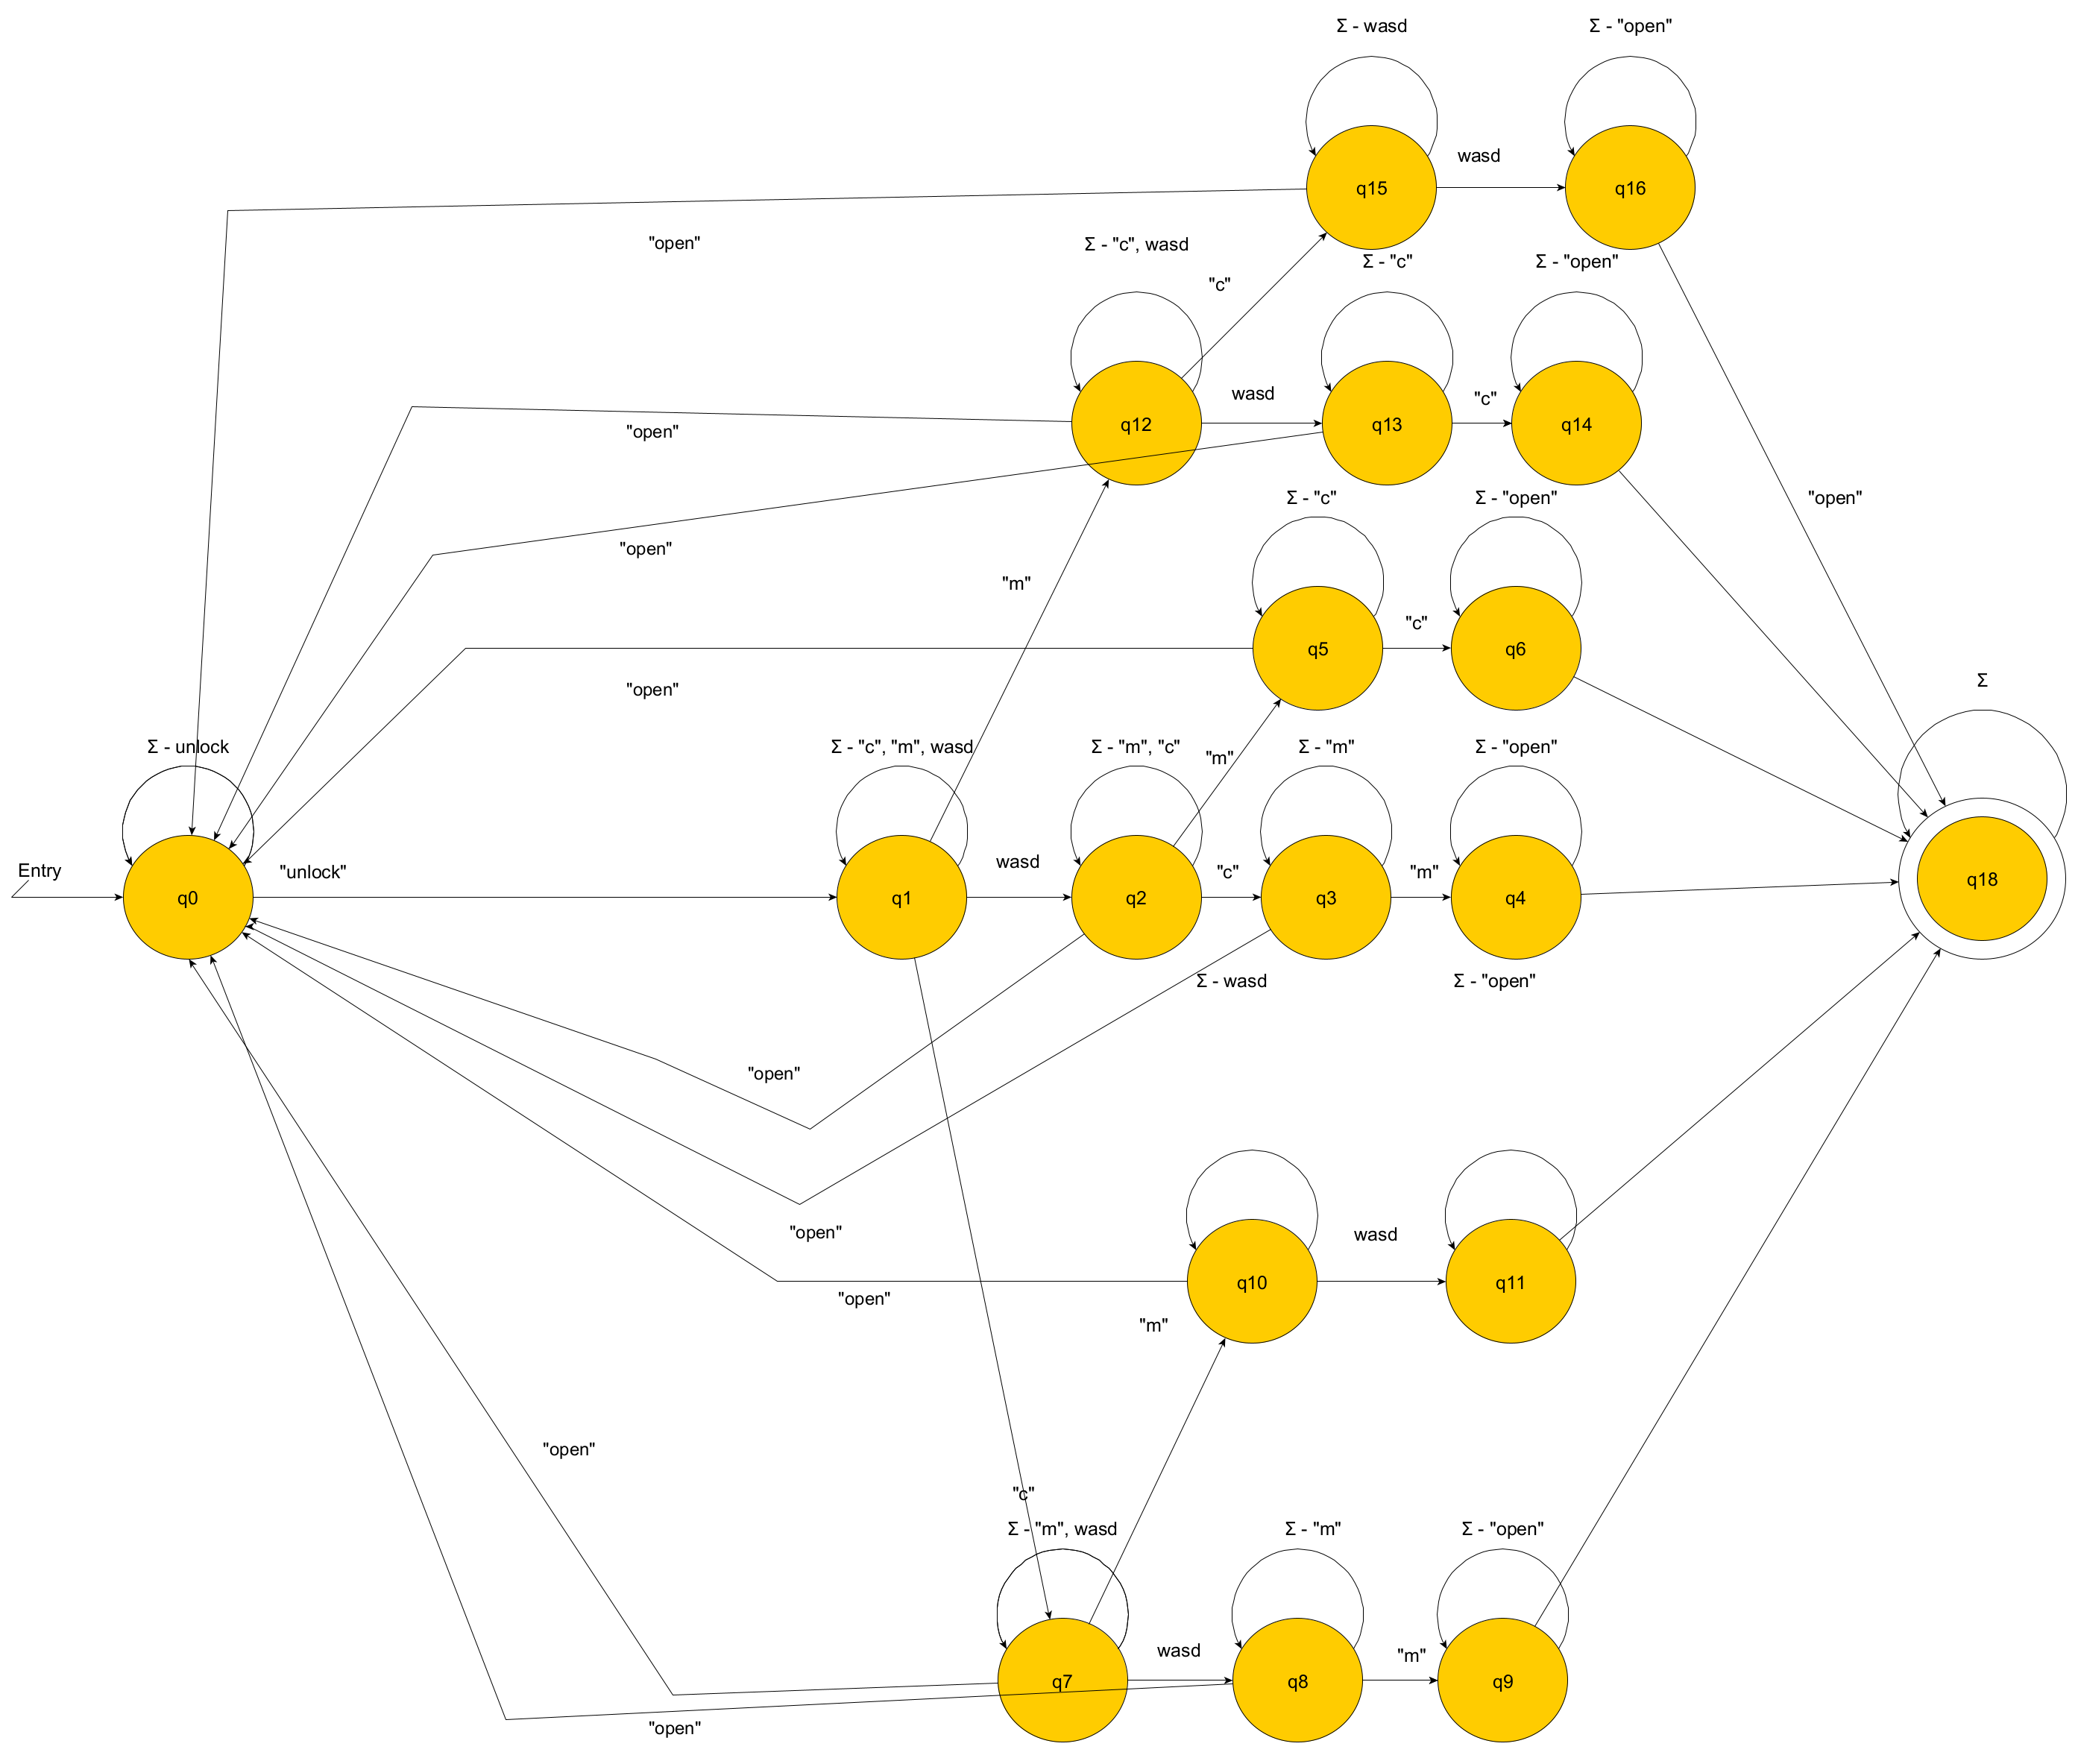
\includegraphics[width=\textwidth,height=\textheight,keepaspectratio]{../dfa.png}}

We have 18 finite set of states and in our alphabet we have "open" , "wasd", "c", "m" and "unlock" 
On step one Q0 you have to write unlock if not you will remain in Q0
After you have arrived  in Q1 you have the choice in between wasd, c, m because in able to unlock the secret door you must c, craft then m, mine or wasd to move in any order that's why after Q1 it divides in 3 because the order is not important.
If you type a move command (w,a,s or d) you enter Q2, the only options you have from now are mine or craft if not you stay in Q2 unless you type open which sends you back to Q0 and have to start again. If you type c you go into Q3 so the last thing you have to write is mine if you write anything else you stay in Q3 expect "open" which sends you in Q0 after mining you enter Q4. From there your only option is to "open" which unlocks the secret door.
Now because the order doesn't matter after Q2  you can also type m for mine which sends you in Q5 where the only option is c, "craft" if you type anything else you go back to Q0 after you type C you entre Q6 where you can only type "open" which will unlock the secret door.
We have created 2 other branches based on the same principal so we can cover all the possible ways you can acces the secret door

Note: in our alphabet "wasd" stands for "w", "a", "s" or "d" 
